% -*- root: ../main.tex -*-

% Devono essere esposte le scelte progettuali operate nelle varie fasi di sviluppo dell'elaborato. In questa sezione devono essere documentati gli schemi di progetto relativamente all'architettura complessiva del sistema e alle sue componenti di rilievo che possano meritare un'analisi di dettaglio. Per le componenti software si può ricorrere ad esempio a diagrammi delle classi, di sequenza, stato, attività. Per le componenti hardware è possibile includere opportuni schemi in grado di descrivere l'architettura fisica adottata.
% 15000 - 24000 battute 

%Architettura complessiva, descrizione di pattern architetturali usati, componenti del sistema distribuito, scelte tecnologiche cruciali ai fini architetturali -- corredato da pochi ma efficaci diagrammi
%Ricordate che una scelta architetturale può ritenersi giustificata o meno solo a fronte dei requirement che avete indicato; viceversa, ogni requirement "critico" dovrebbe influenzare qualcuna della scelte architetturali effettuate e descritte.
%L'architettura deve spiegare quali sono i sotto-componenti del sistema (da 5 a 15, diciamo), ognuno cosa fa, chi parla con chi e per dirsi cosa -- i diagrammi aiutano, ma poi la prosa deve chiaramente indicare questi aspetti. INDIPENDENTE DALLA TECNOLOGIA
\chapter{Design Architetturale}
    In questo capitolo verrà analizzata l'architettura del sistema ad alto livello cercando di spiegare le scelte effettuate in relazione ai requisiti che sono stati elaborati precedentemente. Lo scopo è quello di esaminare i componenti principali che formano l'applicazione e di come essi comunichino tra loro.

    \section{Architettura Generale}\label{chap:architectural-design}
    L'architettura generale del sistema si basa sul pattern \textbf{Model View Controller} (MVC) per rendere il più possibile modulari e separati i compiti svolti da ciascun componente. In particolare, è stato scelto di separare ulteriormente i ruoli di \textit{view} e \textit{controller} creando delle coppie di essi per ciascuna pagina dell'applicazione. In questo modo il comportamento di ciascuna pagina risulta completamente separato dalle altre, così permettendo possibili modifiche o funzionalità non previste durante la fase di progettazione. Questo è stato gestito attraverso un "AppController", che contiene al suo interno la coppia di \textit{controller} e \textit{view} della pagina attualmente caricata e mette a disposizione il necessario per navigare da una pagina all'altra.
    
    \begin{figure}[H]
        \centering
        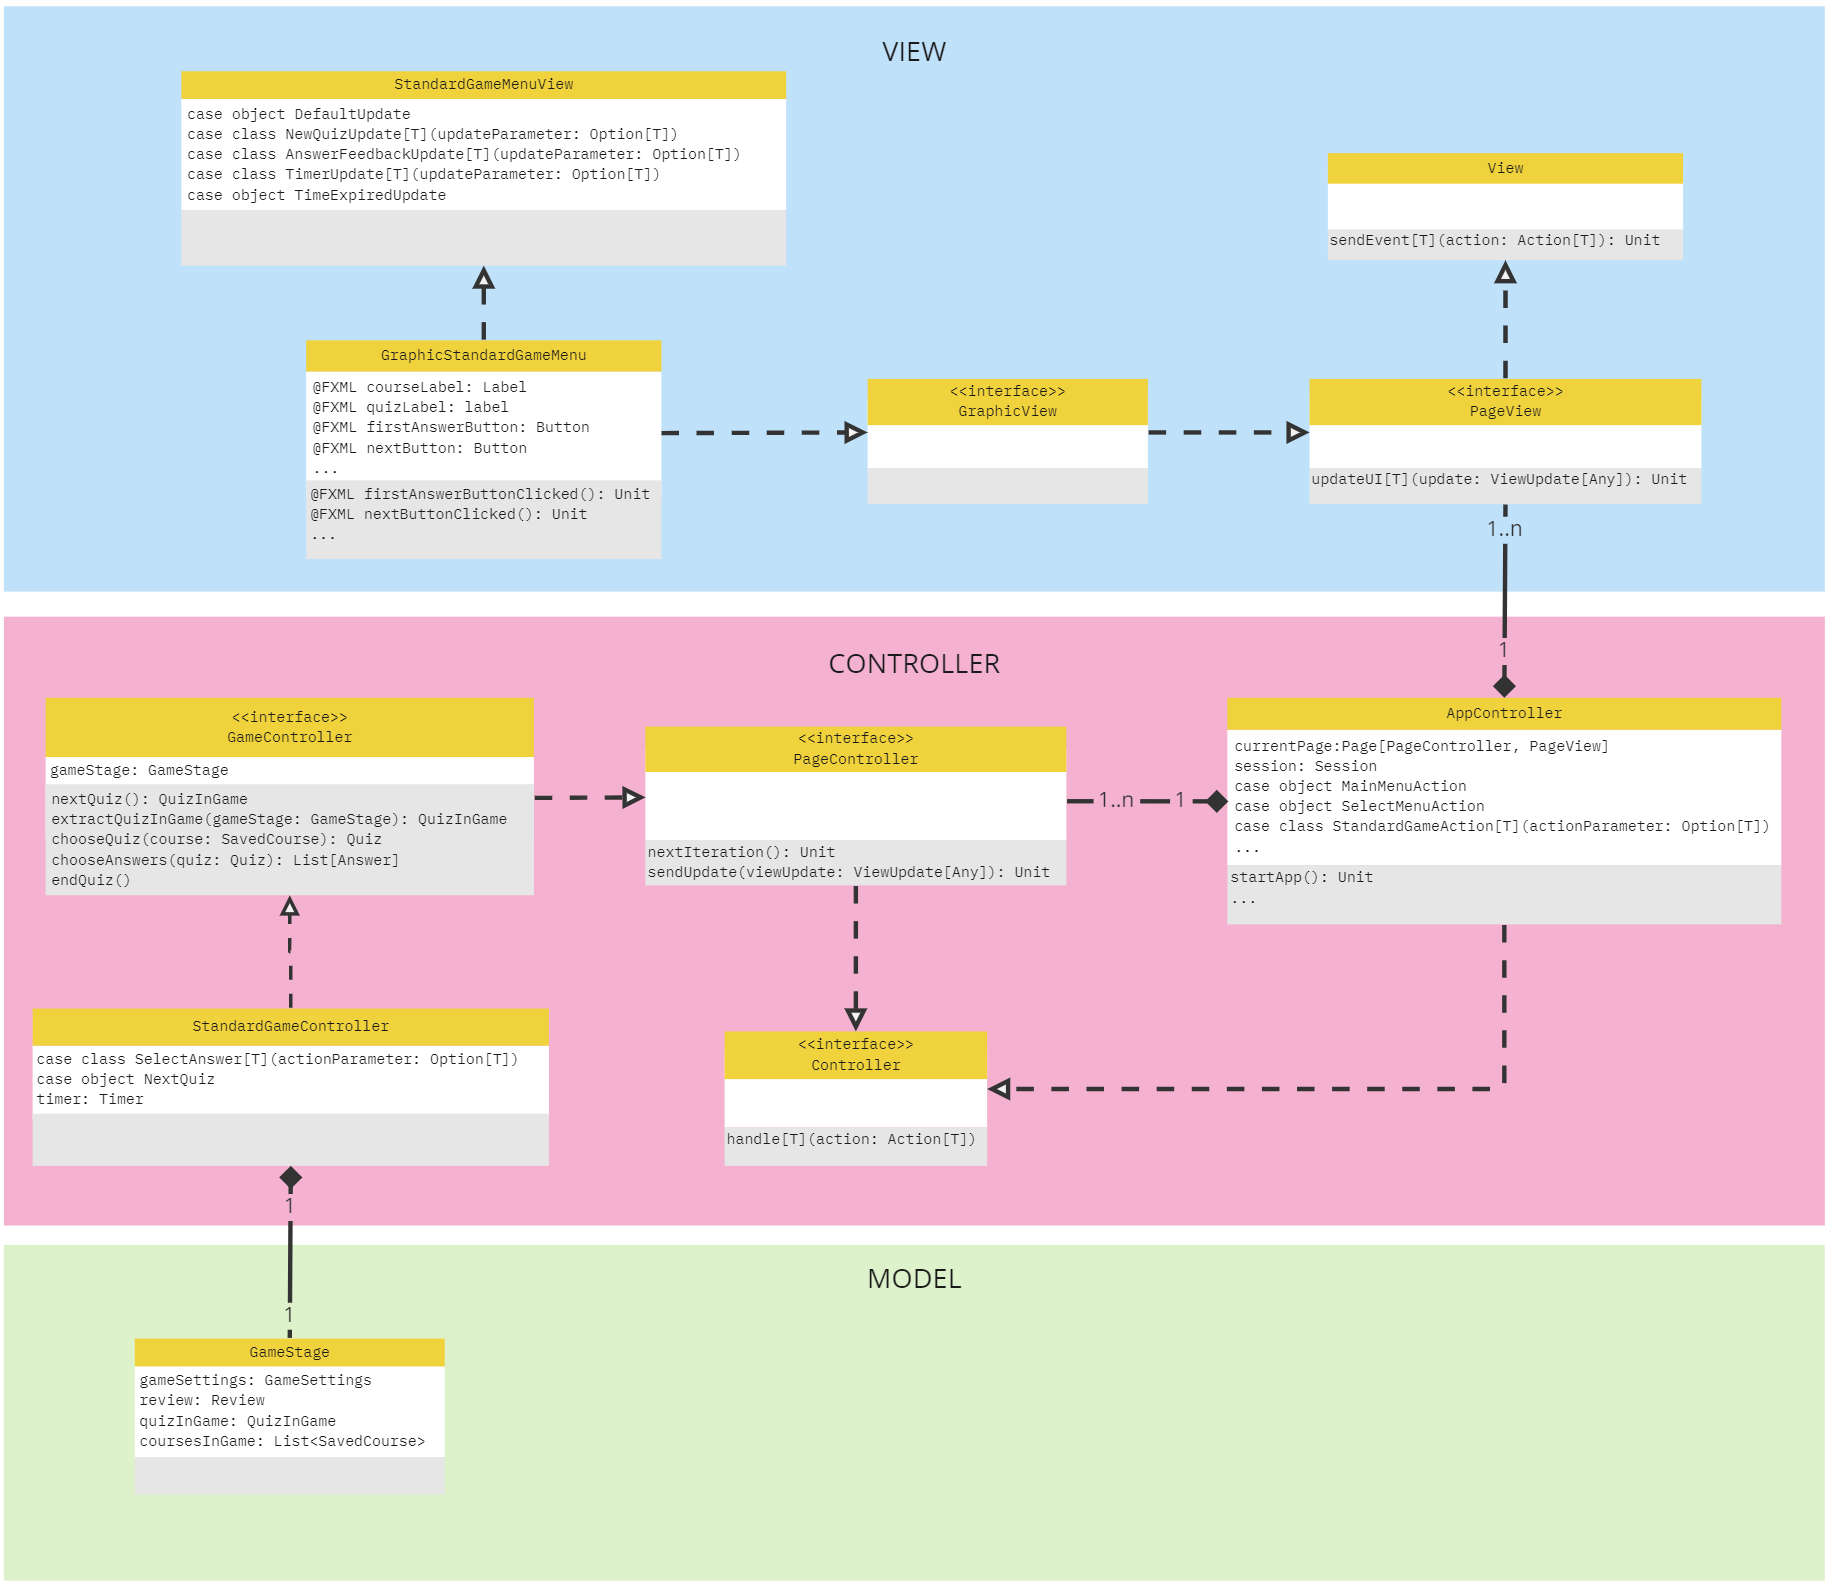
\includegraphics[width=\textwidth]{Miro/general_architecture.png}
        \caption{Architettura generale dell'applicazione}
        \label{fig:mvc-generale}
    \end{figure}
    
    \subsection{View}
        Nell'architettura realizzata, il componente "View" si occupa della comunicazione con il \textit{controller} inviando ad esso le azioni che un utente effettua sull'interfaccia grafica. Ciascuna pagina dell'applicazione deve estendere l'interfaccia generale "PageView", la quale definisce un metodo per l'aggiornamento della pagina stessa a seguito della ricezione di aggiornamenti da parte del \textit{controller} della pagina corrispondente. "GraphicView" estende una "PageView" aggiungendo tutti i comportamenti comuni relativi ad una GUI. Essa viene a sua volta estesa da ciascuna implementazione delle interfaccie grafiche di ciascuna pagina (nella Figura \ref{fig:mvc-generale} è riportato come esempio solamente l'implementazione della \textit{view} relativa ad una partita standard). Avendo scelto di utilizzare JavaFX per realizzare l'interfaccia grafica dell'applicazione, tali classi di implementazione assumono il ruolo di FXControllers delle GUI. Ogni implementazione di una interfaccia grafica di una pagina (ad esempio "GraphicStandardGameMenu") deve anche estendere una \textit{view} specifica della pagina ("StandardGameMenuView"), la quale contiene tutti i possibili aggiornamenti su una generica interfaccia grafica relativa a tale pagina. In questo modo, una specifica implementazione deve sia soddisfare i vincoli imposti da una generica tipologia di interfaccia grafica sia gestire gli aggiornamenti specifici da effettuare su quella pagina.
        
    \subsection{Controller}\label{chap:generic-controller}
        Come precedentemente accennato, l'unione e la comunicazione tra la \textit{view} e il \textit{controller} di una specifica pagina viene gestita tramite "AppController", il quale mantiene il riferimento ad essi. "AppController" permette la navigazione tra le pagine andando a modificare la pagina attualmente in uso.
        Ogni \textit{controller} di una pagina deve estendere l'interfaccia "PageController", la quale impone l'esecuzione di una iterazione successiva e l'invio di update all'interfaccia grafica. L'interfaccia "Controller" specifica una generica funzione di gestione delle azioni eseguite da un utente.
        Una "PageView" compone, insieme ad un "PageController", una pagina completamente funzionante dell'applicazione e la comunicazione tra \textit{view} e \textit{controller} avviene unicamente attraverso l'invio di azioni e di update. Nel caso della pagina relativa ad una partita, come mostrato in Figura \ref{fig:mvc-generale}, i comportamenti generali di qualsiasi modalità di partita sono stati astratti in una interfaccia "GameController". Ciascuna modalità di gioco estende "GameController", implementando poi la propria logica specifica e gestendo le possibili azioni di gioco definite nel \textit{controller} di tale modalità.
 
    \subsection{Model}
        Il \textit{model} dell'applicazione è utilizzato quasi completamente per modellare gli oggetti del dominio necessari allo svolgimento di una partita.
        Come in Figura \ref{fig:mvc-generale}, esso viene sintetizzato nel "GameStage", il quale modella tutti gli elementi generali presenti in una partita, ad esempio, le impostazioni di gioco, il riepilogo della partita e i corsi utilizzati durante la partita per estrarre i quiz da porre. "GameStage" viene utilizzato e modificato dal \textit{controller} della modalità di gioco secondo la logica implementata e poi viene comunicato alla \textit{view} per effettuare gli aggiornamenti necessari sull'interfaccia grafica. Come già detto, nell'architettura generale è stata presentata una versione molto riassuntiva del \textit{model}, il quale verrà successivamente dettagliato nella parte di Design di Dettaglio \ref{chap:design}.